L'arbre ci-dessous
\footnote{
	Bien entendu, cet arbre a été obtenu via un programme et non à la main.
}
permet de gagner en un minimum de coups au baseball des couleurs pour trois bases (il y a 33 configurations différentes et dans le pire des cas on peut gagner en cinq coups).
Pour cela, repérer la configuration à résoudre puis suivre les arêtes de la droite vers la gauche pour avoir les mouvements à faire.


\begin{center}
    \begin{tikzpicture}[
    rotate=90,
    level distance=2.5cm,
        level 1/.style={sibling distance=10cm},
        level 2/.style={sibling distance=5cm},
        level 3/.style={sibling distance=2cm},
        level 4/.style={sibling distance=1cm},
        level 5/.style={sibling distance=0.5cm},
    ]
    \node{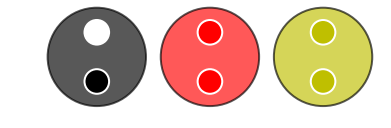
\includegraphics[scale=0.12]{content/optimal/tree_sol/moves/0.png}}
child{node{
\includegraphics[scale=0.12]{content/optimal/tree_sol/moves/1.png}}
child{node{
\includegraphics[scale=0.12]{content/optimal/tree_sol/moves/3.png}}
child{node{
\includegraphics[scale=0.12]{content/optimal/tree_sol/moves/7.png}}
child{node{
\includegraphics[scale=0.12]{content/optimal/tree_sol/moves/16.png}}
child{node{
\includegraphics[scale=0.12]{content/optimal/tree_sol/moves/26.png}}}}
child{node{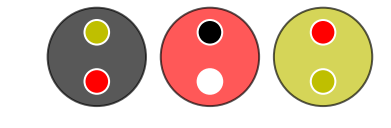
\includegraphics[scale=0.12]{content/optimal/tree_sol/moves/17.png}}
child{node{
\includegraphics[scale=0.12]{content/optimal/tree_sol/moves/27.png}}}}}
child{node{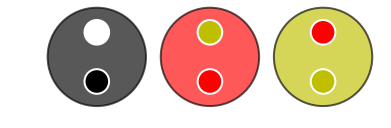
\includegraphics[scale=0.12]{content/optimal/tree_sol/moves/8.png}}}
child{node{
\includegraphics[scale=0.12]{content/optimal/tree_sol/moves/9.png}}
child{node{
\includegraphics[scale=0.12]{content/optimal/tree_sol/moves/18.png}}
child{node{
\includegraphics[scale=0.12]{content/optimal/tree_sol/moves/28.png}}}
child{node{
\includegraphics[scale=0.12]{content/optimal/tree_sol/moves/29.png}}}}
child{node{
\includegraphics[scale=0.12]{content/optimal/tree_sol/moves/19.png}}
child{node{
\includegraphics[scale=0.12]{content/optimal/tree_sol/moves/30.png}}}}}}
child{node{
\includegraphics[scale=0.12]{content/optimal/tree_sol/moves/4.png}}
child{node{
\includegraphics[scale=0.12]{content/optimal/tree_sol/moves/10.png}}
child{node{
\includegraphics[scale=0.12]{content/optimal/tree_sol/moves/20.png}}}}
child{node{
\includegraphics[scale=0.12]{content/optimal/tree_sol/moves/11.png}}
child{node{
\includegraphics[scale=0.12]{content/optimal/tree_sol/moves/21.png}}}}}}
child{node{
\includegraphics[scale=0.12]{content/optimal/tree_sol/moves/2.png}}
child{node{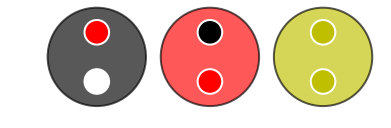
\includegraphics[scale=0.12]{content/optimal/tree_sol/moves/5.png}}
child{node{
\includegraphics[scale=0.12]{content/optimal/tree_sol/moves/12.png}}}
child{node{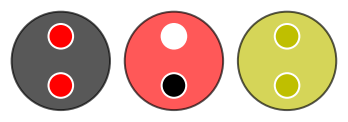
\includegraphics[scale=0.12]{content/optimal/tree_sol/moves/13.png}}
child{node{
\includegraphics[scale=0.12]{content/optimal/tree_sol/moves/22.png}}}}}
child{node{
\includegraphics[scale=0.12]{content/optimal/tree_sol/moves/6.png}}
child{node{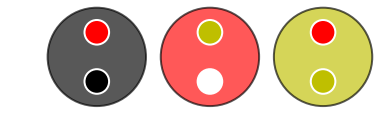
\includegraphics[scale=0.12]{content/optimal/tree_sol/moves/14.png}}
child{node{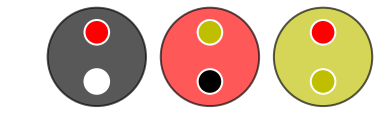
\includegraphics[scale=0.12]{content/optimal/tree_sol/moves/23.png}}}
child{node{
\includegraphics[scale=0.12]{content/optimal/tree_sol/moves/24.png}}
child{node{
\includegraphics[scale=0.12]{content/optimal/tree_sol/moves/31.png}}}}}
child{node{
\includegraphics[scale=0.12]{content/optimal/tree_sol/moves/15.png}}
child{node{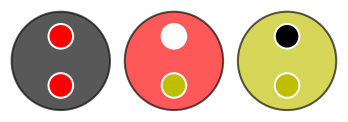
\includegraphics[scale=0.12]{content/optimal/tree_sol/moves/25.png}}
child{node{
\includegraphics[scale=0.12]{content/optimal/tree_sol/moves/32.png}}}}}}};
    \end{tikzpicture}
\end{center}

